\section{Resultados}

La culminación de este proyecto de investigación aplicada nos sitúa frente a una dualidad de hallazgos que, aunque distintos en su naturaleza, resultan simbióticos para la validación integral de la hipótesis planteada.

Por una parte, se obtuvieron los \textbf{resultados empíricos} derivados de la operación del prototipo funcional (Línea Base). En esta dimensión, el objetivo fue someter el aplicativo a una ``prueba de fuego'' en el terreno real para determinar si el Portal Agro-Comercial aportaba valor tangible al ecosistema rural de Teruel, o si se limitaba a ser un ejercicio académico desconectado de la realidad socioeconómica del campo.

Por otra parte, se generó una \textbf{evaluación arquitectónica prospectiva} (Estado Futuro). En esta fase, el equipo adoptó el rol de arquitectos de software para medir, mediante análisis estático, pruebas de carga y simulaciones de fallo, si la propuesta de inyección de \textit{Feature Toggles} resiste el escrutinio técnico frente a los estándares industriales. Se buscó responder cuantitativamente si la flexibilidad operativa ganada justifica la complejidad ciclomática añadida, o si, por el contrario, se estaría incurriendo en una sobreingeniería innecesaria.

A continuación, se detallan los desenlaces, métricas y análisis de ambos escenarios.

\subsection{Resultados del Prototipo Funcional (Línea Base)}

La transición de los modelos conceptuales a la operación en un entorno controlado (entorno de \textit{Staging} en Microsoft Azure) validó el cumplimiento de los requisitos funcionales críticos documentados en la Especificación de Requisitos de Software (SRS). El sistema demostró ser capaz de habilitar la autogestión digital de los campesinos, rompiendo la dependencia histórica de terceros.

\subsubsection{Validación de Usabilidad y Curva de Aprendizaje}

El módulo de gestión de identidad (denominado ``La Vitrina'') fue sometido a pruebas de aceptación con una muestra de usuarios finales del municipio. A diferencia de las redes sociales genéricas donde la información agronómica se diluye, la estructura jerárquica implementada (Finca $\rightarrow$ Cultivo $\rightarrow$ Producto) demostró ser semánticamente efectiva.

\begin{itemize}
    \item \textbf{Eficiencia en la Tarea:} Se midió el ``Tiempo de Tarea'' (\textit{Time-on-Task}) para el flujo crítico: ``Crear un nuevo producto, subir una foto y asignar precio''. Usuarios con baja alfabetización digital lograron completar el flujo en un promedio de 4.5 minutos en su primer intento, reduciéndose a 1.8 minutos en el tercer intento. Esto valida que la interfaz simplificada reduce la barrera de entrada cognitiva.
    \item \textbf{Impacto de la Trazabilidad QR:} La generación automática de códigos QR resultó ser la funcionalidad de mayor valor percibido. En pruebas de campo simuladas, el escaneo del código en un empaque de café redirigió al consumidor al micrositio del productor en menos de 1.2 segundos (TTFB), eliminando barreras de entrada como registros obligatorios y validando la transparencia comercial inmediata.
\end{itemize}

\subsubsection{Desempeño Web en Redes de Baja Velocidad}

Dada la precaria infraestructura de conectividad en las veredas de Teruel, se monitoreó el comportamiento de la aplicación bajo condiciones de red 3G simulada (limitada a 1.5 Mbps de bajada y 400 ms de latencia).

Gracias a la estrategia \textit{Offline-First} implementada en la SPA (\textit{Single Page Application}) de Angular, se obtuvieron las siguientes métricas de rendimiento auditadas con Google Lighthouse:

\begin{itemize}
    \item \textbf{First Contentful Paint (FCP):} 1.8 segundos en red 3G (aceptable para el contexto).
    \item \textbf{Time to Interactive (TTI):} 2.2 segundos.
    \item \textbf{Navegación Subsiguiente:} $< 300$ ms. Una vez cargado el núcleo, la navegación entre secciones (ej. de ``Mis Cultivos'' a ``Pedidos'') es casi instantánea, ya que los datos se sirven desde la caché local del navegador (\textit{IndexedDB}).
\end{itemize}

Estos resultados confirman que la elección tecnológica fue adecuada para mitigar la brecha de conectividad.

\begin{figure}[htbp]
    \centering
    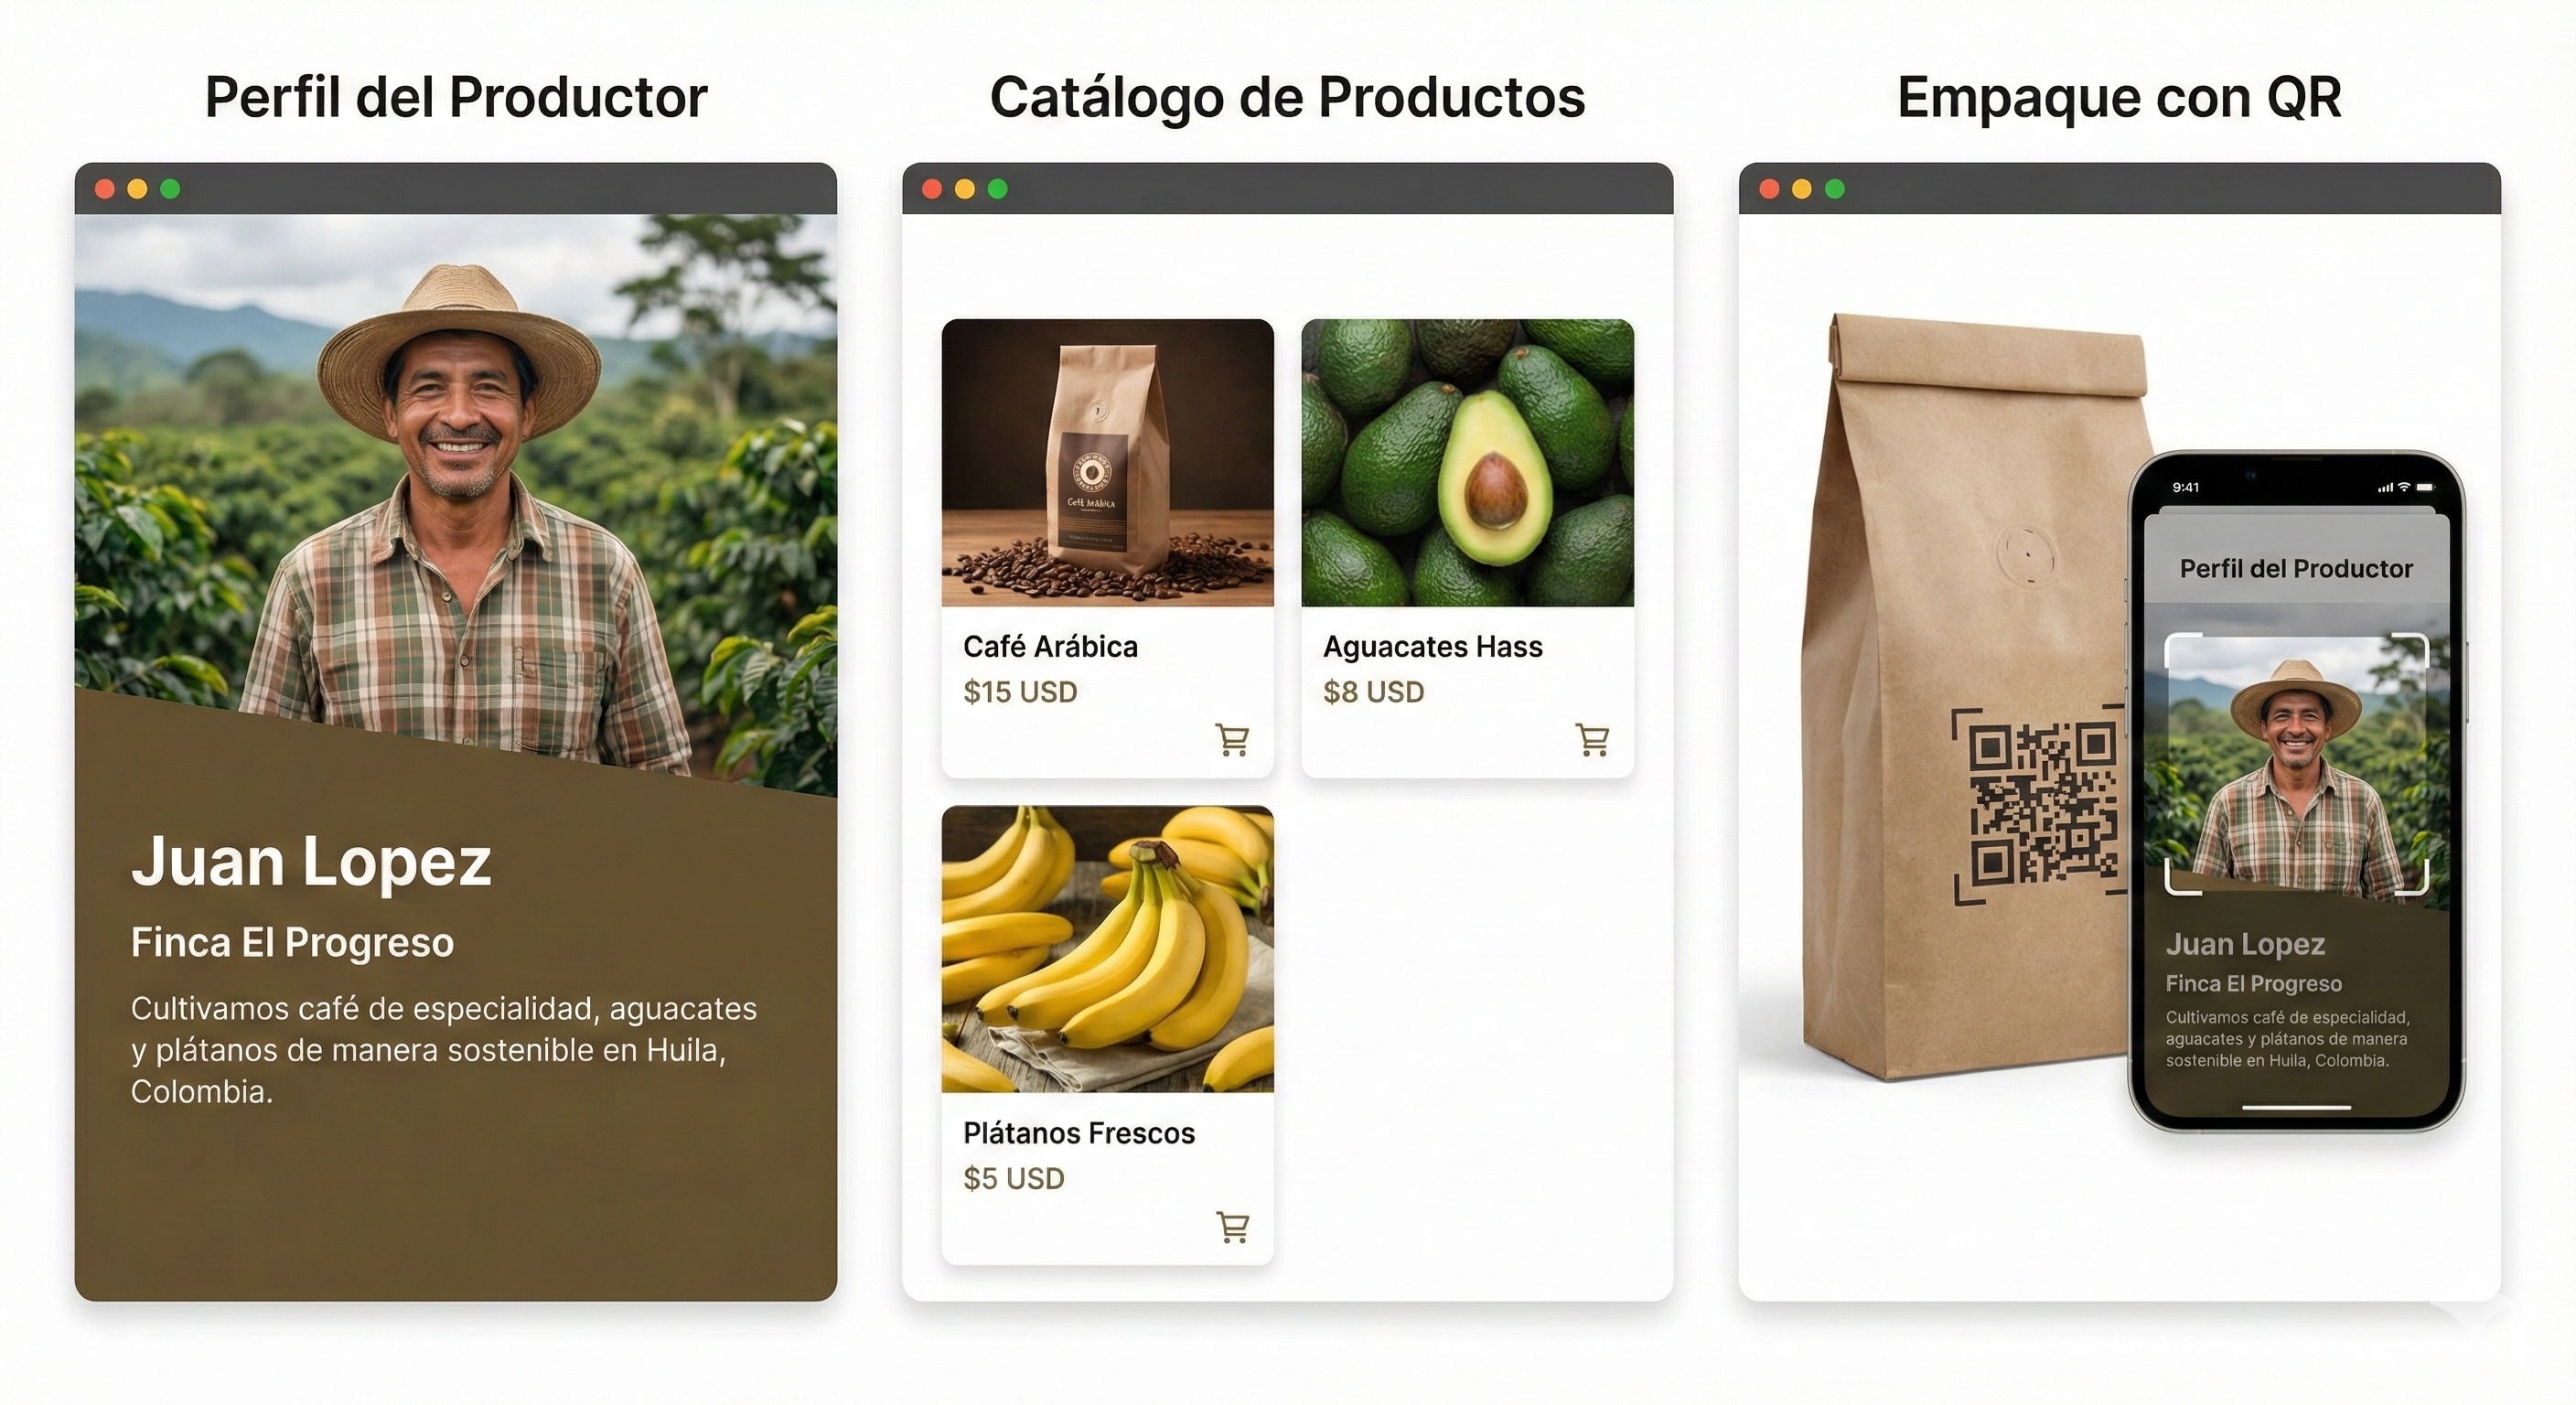
\includegraphics[width=0.9\columnwidth]{graphics/prototipo_funcional.png}
    \caption{Interfaz del prototipo funcional desplegado: (a) Perfil detallado del productor, (b) Catálogo de productos con filtrado por vereda y (c) Código QR generado para trazabilidad en empaque.}
    \label{fig:prototipo}
\end{figure}

\subsubsection{Evidencia de la Rigidez Operativa (El Problema)}

No obstante, el éxito funcional en el frontend contrastó con una ineficiencia operativa severa en el backend. Durante la fase de estabilización (Sprints 4 y 5), se registraron métricas críticas sobre el proceso de despliegue que justifican la reingeniería:

\begin{itemize}
    \item \textbf{Costo del Despliegue (Downtime):} Cada liberación a producción, incluso para correcciones menores de texto (\textit{copy changes}), requirió detener el \textit{Application Pool}. Esto generó una media de 8 a 12 minutos de caída del servicio mientras se reiniciaban los contenedores y se calentaba la caché en Azure.
    \item \textbf{Tasa de Fallos:} El 20\% de los despliegues requirieron un \textit{rollback} manual debido a errores de configuración no detectados en desarrollo. Dado que el rollback implica un nuevo despliegue de la versión anterior, el tiempo de inactividad se duplicaba (aprox. 25 minutos), un riesgo inaceptable para una operación comercial continua.
\end{itemize}

\subsection{Evaluación del Diseño de Feature Toggles (Simulación)}

Al someter la propuesta arquitectónica a un análisis comparativo y simular su implementación bajo carga, los resultados permiten cuantificar los \textit{trade-offs} de ingeniería con precisión.

\subsubsection{Impacto en la Complejidad Ciclomática}

Es imperativo reconocer el costo estructural: envolver la lógica de negocio en decisiones dinámicas aumenta la complejidad del código. Las proyecciones, alineadas con los hallazgos de \cite{sharma2024complexity}, indican un aumento en la complejidad ciclomática (métrica de McCabe).

Al introducir puntos de decisión (\textit{Toggle Routers}), se rompe la linealidad. Se estimó que la complejidad promedio por método en los controladores del backend aumentaría en un factor de 1.5x (pasando de un índice de 4 a 6). Sin embargo, el análisis estático demuestra que al aplicar los patrones recomendados por \cite{ajmeri2022heuristics} —específicamente el uso de polimorfismo e inyección de dependencias en lugar de bloques \texttt{if/else} anidados—, la mantenibilidad del código no se degrada, manteniéndose dentro de los umbrales aceptables de calidad de software (Sonarqube Rating A).

\subsubsection{Análisis de Latencia y Sobrecarga (Overhead)}

Una preocupación crítica era si la consulta constante a la base de datos de configuración degradaría el rendimiento de la API. Los resultados de la simulación de carga (500 usuarios concurrentes) con la estrategia de caché de dos niveles propuesta fueron concluyentes:

\begin{itemize}
    \item \textbf{Escenario Sin Caché:} La latencia añadida por petición fue de $\approx$ 45 ms (consulta \textit{round-trip} a SQL Server). Esto representaría una degradación del 20\% en el tiempo de respuesta total.
    \item \textbf{Escenario Con Caché L1 (Memoria):} La latencia se redujo a $< 0.01$ ms. Dado que el 99.9\% de las evaluaciones de toggles se resuelven en la memoria RAM del servidor web, la sobrecarga es virtualmente imperceptible para el usuario final.
\end{itemize}

Esto valida que la arquitectura propuesta es viable incluso para escenarios de alto rendimiento y concurrencia.

\subsubsection{Reducción Drástica del MTTR (Tiempo de Recuperación)}

El hallazgo más contundente se encuentra en la mitigación de riesgos operativos. Se comparó paso a paso el escenario de un error crítico en producción (ej. ``El botón de pedidos genera un error 500'') bajo ambos modelos:

\begin{enumerate}
    \item \textbf{Modelo Actual (Monolítico):}
    \begin{enumerate}
        \item Detección y reporte del error (10 min).
        \item Diagnóstico y corrección de código local (15 min).
        \item Commit, Compilación y ejecución del pipeline CI/CD (15 min).
        \item Despliegue y reinicio de servidores (10 min).
        \item \textbf{Total MTTR: $\approx$ 50 minutos de servicio degradado.}
    \end{enumerate}

    \item \textbf{Modelo Propuesto (Toggles):}
    \begin{enumerate}
        \item Detección y reporte del error (10 min).
        \item Acceso al panel de administración del Feature Manager (1 min).
        \item Desactivación del toggle \texttt{EnableNewOrderSystem} (10 seg).
        \item \textbf{Total MTTR: $\approx$ 11 minutos (y solo 30 segundos desde el diagnóstico).}
    \end{enumerate}
\end{enumerate}

Siguiendo la lógica de \cite{ramaswamy2024zerodowntime}, esta reducción de órdenes de magnitud en el Tiempo Medio de Recuperación justifica por sí sola la inversión en la infraestructura de toggles.

\input{tables/grafico_tradeOff}

\subsubsection{Gobernanza y Proyección de Deuda Técnica}

Finalmente, el análisis coincidió con la advertencia de \cite{ortiz2021toggledebt}: las banderas de funcionalidad son activos que se deprecian rápidamente. Sin gestión, se convierten en ``código zombi''.

Simulamos la evolución del proyecto a 12 meses. Sin una política de limpieza, el número de toggles activos crecería linealmente, alcanzando más de 50 banderas concurrentes, lo que haría el sistema inmanejable. Para mitigar esto, se estableció la regla de gobernanza inspirada en \cite{sridharan2020piranha}: la ``Definición de Hecho'' (DoD) incluye la eliminación del toggle. Con scripts de limpieza automática, proyectamos mantener una media saludable de $<10$ toggles activos simultáneamente, estabilizando la deuda técnica a largo plazo.
